\chapter{Funzioni}

\begin{esercizio}[(10/06/2019 n°6)\footnotemark]
   Calcolare lo scarto quadratico medio della posizione per la funzione d'onda
   \begin{equation*}
      \psi(x)=\int_{-\infty}^{+\infty} \dd{k} e^{ ikx - \lambda|k| } 
   \end{equation*}
\end{esercizio}
\begin{soluzione}
   \footnotetext{Non è esattamente quell'esercizio: per semplificare i conti si è omesso un fattore 4 ad esponente.}
   Il testo ci chiede di calcolare lo scarto quadratico medio della posizione, cioè
   \begin{equation*}
      \sigma_x=\sqrt{\expval*{\hat{x}^2} - \expval*{\hat{x}}^2}
   \end{equation*}
   Dobbiamo calcolare $\expval*{\hat{x}^2}$ e $\expval*{\hat{x}}^2$. Per farlo abbiamo almeno tre modi diversi:
   \begin{enumerate}
      \item Calcoliamo esplicitamente l'integrale con cui è definita $\psi(x)$. In tal caso $\hat{x}$ sarà un operatore\footnote{Attenzione che tale operatore è leggermente diverso dall'operatore $\hat{x}$ che agisce sugli stati $\ket*{\psi}$ di uno spazio di Hilbert, in quanto questo agisce sugli elementi di uno spazio di funzioni. Formalmente si ha però poi una corrispondenza 1:1.} moltiplicativo tale che $\hat{x}\psi(x)=x\psi(x)$, dove $\psi(x)$ sarà una funzione espressa in una forma non integrale;
      \item Calcoliamo tali valori direttamente in questa rappresentazione. L'operatore $\hat{x}$ agirà sulla funzione esattamente come nel caso precedente, quindi quando calcoliamo $\expval*{\hat{x}}$ avremo
      \begin{equation*}
         \expval*{\hat{x}}=\int_{-\infty}^{+\infty} \dd{x} \psi^* \hat{x} \psi
      \end{equation*}
      e in tale espressione dovremo riportare i due integrali di $\psi^*$ e $\psi$, fare il cambio di ordine di integrazione e risolvere tutto in maniera integrale;
      \item Passiamo allo spazio degli impulsi tramite la trasformata di Fourier: scriviamo (ponendo $k=\frac{p}{\hbar}$)
      \begin{equation*}
         \psi(x)
         =\int_{-\infty}^{+\infty} \dd{\qty(\frac{p}{\hbar})} e^{ i\frac{px}{\hbar} - \lambda\qty|\frac{p}{\hbar}| }
         =\frac{1}{\hbar} \int_{-\infty}^{+\infty} \dd{p} e^{ i\frac{px}{\hbar} - \lambda\frac{|p|}{\hbar} }
      \end{equation*}
      da cui deduciamo che la funzione d'onda nello spazio degli impulsi sarà
      \begin{equation*}
         \tilde{\psi}(p)=Ne^{- \lambda\frac{|p|}{\hbar}}
      \end{equation*}
      con $N$ coefficiente di normalizzazione (in cui viene incluso il fattore $1/\hbar$).
   \end{enumerate}
   Adoperiamo la terza possibilità. L'unico svantaggio di questa strada è che in questa rappresentazione l'operatore $\hat{x}$ è un operatore differenziale anziché un operatore moltiplicativo, cioè se vogliamo lavorare nella rappresentazione degli impulsi avrà forma
   \begin{equation*}
      \hat{x}=i\hbar\dv{p}
   \end{equation*}
   Osserviamo però che la funzione d'onda nello spazio degli impulsi è un esponenziale (a meno del valore assoluto), e sappiamo che gli operatori differenziali agiscono sugli esponenziali come degli operatori moltiplicativi, nel senso che quando deriviamo l'esponenziale otteniamo semplicemente la stessa funzione moltiplicata per il coefficiente ad esponente. Quindi in questo caso lavorare con un operatore differenziale non rappresenta un problema.\\
   Per prima cosa, dato che dobbiamo calcolare delle medie, dobbiamo normalizzare la funzione d'onda. Normalizziamo tale funzione nello spazio degli impulsi. Se la normalizziamo in tale spazio, non dobbiamo porci il problema della conversione, perché la stiamo normalizzando direttamente. Ne segue che non ci sono fattori $2\pi\hbar$ da tenere in considerazione\footnote{Tale fattore ci sarebbe stato se avessimo normalizzato $\psi(x)$ e poi avessimo dovuto cercare una normalizzazione di $\tilde{\psi}(p)$, senza fare una nuova ri-normalizzazione. A livello pratico non cambia niente, semplicemente nei due casi troveremo un valore diverso per la costante di normalizzazione.}.\\
   Dobbiamo quindi porre
   \begin{equation*}
      \begin{split}
         1
         & =\int_{-\infty}^{+\infty} \dd{p} |\tilde{\psi}(p)|^2
         =|N|^2 \int_{-\infty}^{+\infty} \dd{p} e^{-2\frac{\lambda|p|}{\hbar}}
         \\
         & =2|N|^2 \int_{0}^{+\infty} \dd{p} e^{-2\frac{\lambda p}{\hbar}}
         =2|N|^2\frac{\hbar}{2\lambda}=\frac{\hbar|N|^2}{\lambda}
         \implies
         N=\sqrt{\frac{\lambda}{\hbar}}
      \end{split}
   \end{equation*}
   dove il secondo passaggio (in cui abbiamo tolto il valore assoluto) è giustificato dal fatto che la funzione d'onda ha il seguente andamento:
   \begin{figure}[H]
      \centering
      \begin{tikzpicture}[scale=.8]
         \draw[->] (-4.2,0) -- (4.2,0) node[right] {$p$};
         \draw[->] (0,-.6) -- (0,3.2) node[above] {$\tilde{\psi}(p)$};
         \draw[color=teal, thick,join=round] plot[smooth, domain=-4:0] (\x,{2.5*exp(\x)}) -- plot[smooth, domain=0:4] (\x,{2.5*exp(-\x)});
         \end{tikzpicture}
   \end{figure}
   il quale è semplicemente un esponenziale decrescente per $p>0$ mentre per $p<0$ è un esponenziale crescente, che nei fatti è la stessa funzione riportata specularmente. Ciò significa le due regioni sono simmetriche, dunque è possibile dividere l'integrale in due parti, una che va da 0 a $+\infty$ e una che va da 0 a $-\infty$, le quali sono identiche e pertanto possiamo considerarne una soltanto e moltiplicare per 2.\\
   Passiamo al calcolo di $\expval*{\hat{x}}$. Ricordiamo che, avendo scelto di normalizzare a 1 nello spazio degli impulsi, per restare coerenti negli integrali che seguono non dovremo mettere un fattore $2\pi\hbar$ a dividere nella misura di integrazione.
   \begin{equation*}
      \expval*{\hat{x}}
      =\int_{-\infty}^{+\infty} \dd{p} \tilde{\psi}^* \hat{x} \tilde{\psi}
      =i\hbar \int_{-\infty}^{+\infty} \dd{p} \tilde{\psi}^* \dv{\tilde{\psi}}{p}
   \end{equation*}
   Notiamo che è lecito scrivere tale espressione, in quanto la funzione è continua in $p=0$ mentre la derivata prima è discontinua, pertanto un'eventuale delta di Dirac figurerebbe soltanto nella derivata seconda. In particolare, la derivata prima è pari a
   \begin{equation*}
      \dv{\tilde{\psi}}{p}=
      \begin{dcases}
         -N\frac{\lambda}{\hbar}e^{-\frac{\lambda p}{\hbar}} & \text{per } p>0\\
         N\frac{\lambda}{\hbar}e^{\frac{\lambda p}{\hbar}} & \text{per } p<0
      \end{dcases}
   \end{equation*}
   e se adesso moltiplichiamo per la $\tilde{\psi}^*$ abbiamo (ricordiamo che $\tilde{\psi}$ è reale)
   \begin{equation*}
      \psi^*\dv{\psi}{p}=
      \begin{dcases}
         -|N|^2\frac{\lambda}{\hbar}e^{-2\frac{\lambda p}{\hbar}} & \text{per } p>0\\
         |N|^2\frac{\lambda}{\hbar}e^{2\frac{\lambda p}{\hbar}} & \text{per } p<0
      \end{dcases}
   \end{equation*}
   Vediamo se esiste un modo per scrivere con un'unica espressione tale funzione. Per quanto riguarda gli esponenziali è sufficiente utilizzare il modulo di $p$ cioè $|p|$; per il coefficiente (che è uguale in entrambi ma negativo per $p>0$ e positivo per $p<0$) possiamo adoperare la funzione segno, che è pari a $1$ quando il suo argomento assume valori positivi e pari a $-1$ quando il suo argomento assume valori negativi, dunque ha il seguente andamento:
   \begin{figure}[H]
      \centering
      \begin{tikzpicture}
         \draw[->] (0,-1.5) -- (0,1.5) node[above] {$\text{sgn}(p)$};
         \draw[->] (-2,0) -- (2,0) node[right] {$p$};
         \draw[red,thick] (-2,-1) -- (0,-1) node[right,black] {$-1$};
         \draw[red,thick] (0,1) node[left,black] {$1$} -- (2,1);
      \end{tikzpicture}
   \end{figure}
   In definitiva l'espressione cercata è
   \begin{equation*}
      \tilde{\psi}^*\dv{\tilde{\psi}}{p}=-|N|^2 \frac{\lambda}{\hbar} \, \text{sign}(p) e^{-2\frac{\lambda p}{\hbar}}
   \end{equation*}
   la quale ha il seguente andamento:
   \begin{figure}[H]
      \centering
      \begin{tikzpicture}[scale=.8]
         \draw[->] (-4.2,0) -- (4.2,0) node[right] {$p$};
         \draw[->] (0,-3.2) -- (0,3.2) node[above] {$\psi^*\dv{\psi}{p}$};
         \draw[color=teal, thick] plot[smooth, domain=-4:0] (\x,-{2.5*exp(\x)});
         \draw[color=teal, thick] plot[smooth, domain=0:4] (\x,{2.5*exp(-\x)});
         \end{tikzpicture}
   \end{figure}
   Tale funzione è anti-simmetrica rispetto a $p=0$: ne segue che quando ne facciamo l'integrale da $-\infty$ a $+\infty$ quest'ultimo sarà pari a zero:
   \begin{equation*}
      \int_{-\infty}^{+\infty} \dd{p} \tilde{\psi}^* \dv{\tilde{\psi}}{p}=0
   \end{equation*}
   Avevamo modo di sapere sin dall'inizio che tale integrale si sarebbe annullato?\\
   Un primo modo è quello di notare che la funzione è pari, per cui la sua derivata è dispari e dunque il prodotto è dispari; un secondo modo è quello di notare che c'è un fattore $i$ a moltiplicare l'integrale, ma siccome $\expval*{\hat{x}}$ non può essere un numero immaginario\footnote{Il motivo è che, essendo $\hat{x}$ un'osservabile, è un operatore hermitiano, il quale ha autovalori reali e dunque anche le sue medie, essendo quest'ultime somme di autovalori moltiplicati per le relative probabilità.} ci aspettiamo che, essendo la funzione d'onda reale (e quindi chiaramente anche la sua derivata), l'integrale debba essere pari a zero. Attenzione! In generale non è detto che la funzione integranda sia reale.\\
   Calcoliamo adesso $\expval*{\hat{x}^2}$, che possiamo calcolare in due modi. Prima però riscriviamo la derivata prima di $\tilde{\psi}$ nella seguente maniera:
   \begin{equation*}
      \dv{\tilde{\psi}}{p}=-N\frac{\lambda}{\hbar} e^{-\frac{\lambda|p|}{\hbar}} \big[ \vartheta(p) - \vartheta(-p) \big]
   \end{equation*}
   dove l'espressione tra parentesi quadre non è altro che la funzione $\text{sgn}(p)$ (si può infatti vedere che per $p>0$ il primo termine è pari a 1 mentre il secondo è pari a 0, viceversa per $p<0$ il primo è pari a 0 e il secondo a $-1$). Il motivo per cui ci serve questa riscrittura è che se vogliamo calcolare la derivata seconda sappiamo come si deriva la theta.\\
   Vediamo adesso i due modi per calcolare $\expval*{\hat{x}^2}$, che sappiamo essere pari a $\mel*{\psi}{\hat{x}^2}{\psi}$.
  \begin{itemize}[leftmargin=0.5cm]
   \item Modo 1: scriviamo tale espressione come
  \begin{equation*}
   \expval*{\hat{x}^2}
   =\mel*{\psi}{\hat{x}\hat{x}}{\psi}
   =| \hat{x}\ket*{\psi} \hspace{-0.1cm} |^2
  \end{equation*}
  con cui intendiamo che facciamo agire una $\hat{x}$ su $\ket*{\psi}$ e una $\hat{x}$ su $\bra*{\psi}$. In questo modo ci riconduciamo al calcolo del modulo quadro del vettore ottenuto dall'applicazione di $\hat{x}$ su $\ket*{\psi}$. Il vantaggio di questo modo è che così facendo non dovremo calcolare la derivata seconda e quindi non dovremo utilizzare la delta di Dirac.\\
  Calcoliamo la quantità $\hat{x}{\psi}$. Ricordando che nella rappresentazione degli impulsi $\hat{x}$ è pari a $i\hbar\dv{p}$ si ha
  \begin{equation*}
      \hat{x}\tilde{\psi}
      =i\hbar\dv{\tilde{\psi}}{p}
      =-iN\lambda e^{-\frac{\lambda |p|}{\hbar}} \big[ \vartheta(p) - \vartheta(-p) \big]
   \end{equation*}
   Questa sarà la nuova funzione d'onda di cui dobbiamo prenderne il modulo quadro. In particolare, per quanto riguarda il quadrato del termine tra parentesi quadre si ha che esso è pari a 1 (ricordiamo che esso non è altro che la funzione segno, la quale elevata al quadrato fa ovviamente 1). Esplicitamente:
   \begin{equation*}
      \big[ \vartheta(p) - \vartheta(-p) \big]^2
      =\vartheta^2(p) + \vartheta^2(-p) - 2\vartheta(p)\vartheta(-p)
      =\vartheta(p) + \vartheta(-p) + 0
      =1
   \end{equation*}
   in quanto la funzione theta moltiplicata per se stessa resta uguale, mentre nel doppio prodotto abbiamo il prodotto tra due funzioni tali che una è pari a 1 laddove l'altra è nulla e viceversa, quindi tale termine è pari a zero. Infine i due termini che restano sono banalmente pari alla costante 1 per qualsiasi valore di $p$.\\
   In definitiva abbiamo che
   \begin{equation*}
      |\hat{x}\tilde{\psi}|^2=|N|^2 \lambda^2 e^{-2\frac{\lambda |p|}{\hbar}}
   \end{equation*}
   Mettendo tale quantità sotto integrale avremo
   \begin{equation*}
      \expval*{\hat{x}^2}=|N|^2\lambda^2 \int_{-\infty}^{+\infty} \dd{p} e^{-2\frac{\lambda |p|}{\hbar}}
      =2|N|^2 \lambda^2 \frac{\hbar}{2\lambda}
      =2\frac{\lambda}{\hbar} \lambda^2 \frac{\hbar}{2\lambda}
      =\lambda^2
   \end{equation*}
   dove abbiamo adoperato gli stessi passaggi di prima (divisione in due integrali, considerazioni sulla simmetria ecc.)\\
   \item Modo 2: facciamo agire $\hat{x}^2$ su $\tilde{\psi}$ e poi calcoliamo l'integrale di ciò che viene fuori moltiplicato per $\tilde{\psi}^*$. In questo caso sarà necessario adoperare la delta di Dirac.\\
   Stavolta avremo
   \begin{equation*}
      \expval*{\hat{x}^2}
      =\int_{-\infty}^{+\infty} \dd{p} \tilde{\psi}^* \hat{x}^2 \tilde{\psi}
      =-\hbar^2 \int_{-\infty}^{+\infty} \dd{p} \tilde{\psi}^* \dv[2]{\tilde{\psi}}{p}
   \end{equation*}
   quindi dobbiamo calcolare la derivata seconda. Per farlo riscriviamo meglio la derivata prima, moltiplicando le due theta per l'esponenziale e esplicitando i valori assoluti:
   \begin{equation*}
      \dv{\tilde{\psi}}{p}=-N\frac{\lambda}{\hbar} \qty[ e^{-\frac{\lambda p}{\hbar}}\vartheta(p) - e^{\frac{\lambda p}{\hbar}} \vartheta(-p) ]
     \end{equation*}
   La derivata seconda allora sarà
   \begin{equation*}
      \dv[2]{\tilde{\psi}}{p}
      =-\frac{N\lambda}{\hbar} \qty[
         -\frac{\lambda}{\hbar} e^{-\frac{\lambda p}{\hbar}}\vartheta(p)
         -\frac{\lambda}{\hbar} e^{\frac{\lambda p}{\hbar}} \vartheta(-p)
         + e^{-\frac{\lambda p}{\hbar}} \delta(p)
         +e^{\frac{\lambda p}{\hbar}} \delta(p) ]
   \end{equation*}
   dove l'ultimo termine deriva da
   \begin{equation*}
      \dv{p}\vartheta(-p)=\dv{(-p)}{p}\dv{(-p)}\vartheta(-p)=-\delta(-p)=-\delta(p)
   \end{equation*}
   Osserviamo inoltre che gli ultimi due addendi sono entrambi pari semplicemente a $\delta(p)$ per la proprietà secondo cui $f(p)\delta(p)=f(0)\delta(p)$, e l'esponenziale calcolato in 0 è pari a 1; possiamo quindi scrivere
   \begin{equation*}
      \dv[2]{\tilde{\psi}}{p}
      =-\frac{N\lambda}{\hbar} \qty[
         -\frac{\lambda}{\hbar} e^{-\frac{\lambda p}{\hbar}}\vartheta(p)
         -\frac{\lambda}{\hbar} e^{\frac{\lambda p}{\hbar}} \vartheta(-p)
         + \delta(p)
         + \delta(p) ]
      =-\frac{N\lambda}{\hbar} \qty[ -\frac{\lambda}{\hbar} e^{-\frac{\lambda |p|}{\hbar}} + 2\delta(p) ]
   \end{equation*}
   dove abbiamo fatto in un certo senso il passaggio inverso a prima, nel senso che abbiamo messo in evidenza l'esponenziale reintroducendo il valore assoluto e poi abbiamo sfruttato il fatto che $\vartheta(p) + \vartheta(-p)=1$.\\
   A questo punto possiamo calcolare $\expval*{\hat{x}^2}$:
   \begin{equation*}
      \begin{split}
         \expval*{\hat{x}^2}
         & =|N|^2 \lambda \hbar \int_{-\infty}^{+\infty} \dd{p} e^{-\frac{\lambda |p|}{\hbar}} \qty[ -\frac{\lambda}{\hbar} e^{-\frac{\lambda |p|}{\hbar}} + 2\delta(p) ]
         \\
         & =|N|^2 \lambda \hbar \qty{ -\frac{\lambda}{\hbar} \int_{-\infty}^{+\infty} \dd{p} e^{-2\frac{\lambda |p|}{\hbar}} + 2\int_{-\infty}^{+\infty} \dd{p} e^{-\frac{\lambda |p|}{\hbar}} \delta(p) }
         \\
         & =|N|^2 \lambda \hbar \qty{ -\frac{\lambda}{\hbar}\frac{\hbar}{\lambda} + 2 }
         =|N|^2 \lambda \hbar
         =\lambda^2
      \end{split}
   \end{equation*}
   dove il primo integrale lo abbiamo già calcolato in precedenza, mentre per il secondo abbiamo sfruttato il fatto che la $\delta(p)$ messa sotto integrale con un'altra funzione restituisce la funzione calcolata in $p=0$, ma siccome questa in 0 fa 1 l'integrale è semplicemente pari a 1.
   \end{itemize}
   Osserviamo come il risultato sia lo stesso dell'altro caso, perché appunto i due modi sono equivalenti. Vale però la pena notare il seguente fatto: da un punto di vista specificamente fisico, noi stiamo calcolando la media di $\hat{x^2}$, la quale è un numero positivo perché può essere scritta come $| \hat{x}\ket*{\psi} \hspace{-0.1cm} |^2$, che è certamente positivo. Se avessimo escluso il contributo della delta avremmo trovato un valore negativo per $\expval*{\hat{x}}^2$, il che è ovviamente assurdo. Ciò dimostra che bisogna tenere conto in maniera corretta delle discontinuità, altrimenti incappiamo in risultati privi di senso fisico.\\
   In definitiva abbiamo
   \begin{equation*}
      \sigma_x
      =\sqrt{\lambda^2 - 0}
      =\lambda
   \end{equation*}
\end{soluzione}

\newpage

\begin{esercizio}[(14/09/2020 n°1)]
   Un elettrone si trova nello stato descritto in coordinate
   sferiche dalla seguente funzione d'onda:
   \begin{equation*}
      \psi(r,\vartheta,\varphi)=e^{-\frac{\lambda r}{2}} \sin^2{\vartheta}
   \end{equation*}
   Determinare i possibili valori di una misura della componente $L_z$ del momento angolare e le rispettive probabilità. Calcolare poi la probabilità di trovare l'elettrone nella regione dello spazio limitata da entrambe le relazioni $0<r<\frac{1}{\lambda}$ e $0<\vartheta<\frac{\pi}{2}$.
\end{esercizio}
\begin{soluzione}
   Notiamo innanzitutto che il testo ci chiede di calcolare la probabilità, quindi sappiamo già che dovremo normalizzare la funzione d'onda.
   
   La prima richiesta è quella di determinare i possibili valori di una misura $L_z$, ossia di determinare quali siano i possibili autolavori di $\hat{L}_z$. Per tale richiesta non è necessario normalizzare la funzione d'onda, dunque lo faremo in un secondo momento.
   
   In linea di principio, per trovare i valori di $L_z$, dovremmo scrivere la funzione d'onda come una somma di autofunzioni dell'operatore $\hat{L}_z$, dovremmo cioè scrivere $\psi$ come
   \begin{equation*}
      \psi(r,\vartheta,\varphi)=\sum_{n,\ell,m} c_{n,\ell,m} \phi_{n,\ell,m}(r,\vartheta,\varphi)
   \end{equation*}
   dove $\phi_{n,\ell,m}(r,\vartheta,\varphi)$ sono le autofunzioni dell'atomo di idrogeno, che sono autofunzioni anche di $\hat{L}_z$. Dopo aver scritto tale sommatoria dobbiamo andare a vedere quali sono i coefficienti non nulli, in quanto gli stati ad essi corrispondenti saranno quelli in cui la particella può essere misurata e di conseguenza è possibile fare una misura di momento angolare con $L_z=\hbar m$. In altre parole, i possibili valori di una misura di $\hat{L}_z$ sono tutti quei valori per cui il coefficiente è non nullo.

   Ciò vale in generale. In questo caso il problema è molto più semplice perché sappiamo che $\hat{L}_z$ si può esprimere come
   \begin{equation*}
      \hat{L}_z=-i\hbar \pdv{\varphi}
   \end{equation*}
   e siccome la funzione d'onda non dipende da $\varphi$ ha derivata nulla rispetto a quest'ultima, quindi è già autofunzione di $\hat{L}_z$ e pertanto sappiamo già che c'è un solo possibile valore ottenibile da una misura della proiezione del momento angolare, che è $L_z=0$. Inoltre la probabilità è chiaramente pari a 1 perché non possiamo trovare nessun altro valore di $L_z$ e quindi misuriamo $L_z=0$ con probabilità 1.
   
   \vspace{0.2cm}Che sarebbe successo se invece ce ne fossero stati più di uno? Vediamolo facendo due esempi.
   
   \vspace{0.2cm}ES.1 Consideriamo la funzione
   \begin{equation*}
      \chi_1=e^{-\frac{\lambda r}{2}}\sin{\vartheta}( \cos{\varphi} + 2 \sin^2{\varphi} )
   \end{equation*}
   
   Notiamo che la parte $e^{-\frac{\lambda r}{2}}\sin{\vartheta}$ non dipende da $\varphi$, ciò significa che l'informazione su $L_z$ è contenuta nel termine tra parentesi, il quale possiamo riscrivere come
   \begin{equation*}
      \cos{\varphi} + 2 \sin^2{\varphi}
      =\qty[ \frac{e^{i\varphi} + e^{-i\varphi}}{2} - \frac{\qty( e^{i\varphi} - e^{-i\varphi} )^2}{2} ]
      =\frac{1}{2} \qty( 2 + e^{i\varphi} + e^{-i\varphi} - e^{2i\varphi} - e^{-2i\varphi} )
   \end{equation*}
   Quello che abbiamo fatto in sostanza è stato prendere la parte angolare della funzione d'onda, che in questo caso è una generica funzione dipendente da $\varphi$, ed espanderla in una somma di autofunzioni di $\hat{L}_z$.
   
   Tale espansione corrisponde ad avere la somma degli stati
   \begin{equation*}
      2\ket*{0} + \ket*{1} + \ket*{-1} - \ket*{2} - \ket*{-2}
   \end{equation*}
   A questo punto, visto che la probabilità totale deve essere pari a 1, consideriamo la somma dei moduli quadri dei coefficienti dei termini che figurano in tale espressione: essa è pari a $4 + 1 + 1 + 1 +1=8$, dunque dovremo riscrivere lo stato come
   \begin{equation*}
      \frac{1}{\sqrt{8}}\qty( 2\ket*{0} + \ket*{1} + \ket*{-1} - \ket*{2} - \ket*{-2} )
   \end{equation*}
   da cui deduciamo che abbiamo probabilità $\mathbb{P}_0=\frac{4}{8}=\frac{1}{2}$ di misurare $L_z=0$, mentre per tutti gli altri valori la probabilità è pari a $\frac{1}{8}$.
   
   La funzione d'onda $\chi_1$ però non rappresenta il caso più generico, perché è un caso particolare di funzione d'onda del tipo
   \begin{equation*}
      \psi=R(r)\Theta(\vartheta)\Phi(\varphi)
   \end{equation*}
   cioè fattorizzabile nel prodotto di funzioni che dipendono da una sola variabile. Vediamo allora un esempio più generale.

   \vspace{0.2cm} ES.2 Consideriamo la funzione d'onda
   \begin{equation*}
      \chi_2=e^{-\frac{\lambda r}{2}} \sin^2{\vartheta} + e^{-\xi r^2}\cos^2{\varphi}
   \end{equation*}
   Si evince subito che essa non è fattorizzabile a differenza di $\chi_1$.
   Cosa è possibile dire di $L_z$? Innanzitutto riscriviamo la funzione come
   \begin{equation*}
      \chi_2=e^{-\frac{\lambda r}{2}} \sin^2{\vartheta} + 
      \frac{1}{4}e^{-\xi r^2} \qty( e^{2i\varphi} + e^{-2i\varphi} + 2)
   \end{equation*}
   dove abbiamo espanso $\cos^2{\varphi}$ come una somma di autofunzioni di $\hat{L}_z$. Da tale espressione deduciamo che i possibile valori di $L_z$ sono $0,\pm 2 \hbar$ (da notare che il valore $L_z=0$ si poteva dedurre già dal primo addendo, in cui non c'è dipendenza da $\varphi$).

   Se adesso volessimo trovare le probabilità, ciò non sarà semplice come nel caso di $\chi_1$ in cui abbiamo semplicemente letto i coefficienti (ribadiamo che in quel caso era sufficiente leggere i coefficienti perché tutta la dipendenza da $\varphi$ era fattorizza in una sua funzione (la parentesi)). Quello che invece dobbiamo fare in questo caso è svolgere il calcolo esplicito: dopo aver normalizzato la funzione d'onda, la probabilità $\mathbb{P}(L_z=\hbar m)$ di rivelare la particella descritta da questa funzione d'onda con $L_z=\hbar m$ sarà data dalla somma delle probabilità di trovare la particella con una generica energia (cioè un generico valore di $n$), con un generico momento angolare totale (cioè un generico valore di $\ell$) e quel determinato valore di $L_z$, dunque di $m$. In formule:
   \begin{equation*}
      \mathbb{P}(L_z=\hbar m)
      =\sum_{n,\ell} \mathbb{P}(n,\ell,m)
      =\sum_{n,\ell} | \hspace{-0.1cm} \braket*{n,\ell,m}{\psi} \hspace{-0.1cm} |^2
   \end{equation*}
   dove nell'ultimo passaggio abbiamo esplicitato le probabilità come moduli quadri dei prodotti scalari tra lo stato $\ket*{\psi}$ e gli autostati $\ket*{n,\ell,m}$.

   \E\ da notare che, sebbene la sommatoria sia estesa a tutti i valori di $n$ ed $\ell$, nei fatti ci saranno delle probabilità nulle a priori, in quanto se ci mettessimo nella rappresentazione delle posizioni tali probabilità sarebbero date da
   \begin{equation*}
      \sum_{n,\ell} \mathbb{P}(n,\ell,m)
      =\sum_{n,\ell} \qty| \int \dd[3]{\vb*{r}} R_{n,\ell}(r) Y_{\ell,m}^*(\vartheta,\varphi) \psi(r,\vartheta,\varphi) |^2
   \end{equation*}
   e se per esempio volessimo calcolare la probabilità per $m=24$ (il che significa che $\ell$ deve valere almeno 24 e quindi $n$ almeno 25), è chiaro che ci saranno dei termini della sommatoria nulli a prescindere. Esclusi tali termini, il passaggio successivo è esplicitare la dipendenza radiale ed angolare della funzione d'onda, in modo da vedere se si possono operare delle semplificazioni.

   Il problema di questa formula è che se mai si dovesse adoperare nella sua forma più generale, nei fatti dovremmo calcolare un numero potenzialmente infinito di integrali radiali, fatto che potrebbe risultare proibitivo. Per tale ragione, negli esercizi spesso la funzione d'onda ha la forma di un certa funzione $f(r)$ moltiplicata per una somma $g(\vartheta,\varphi)$ di funzioni di $\vartheta$ e $\varphi$. In tal caso la dipendenza radiale è indifferente, perché c'è una singola funzione a moltiplicare e a noi interessa solo la dipendenza angolare, per cui troveremo che la probabilità di trovare la particella con un certo valore di $\ell$ ed $m$ (assumendo che $g(\vartheta,\varphi)$ sia normalizzata) sarà data da
   \begin{equation*}
      \mathbb{P}(\ell,m)
      =\qty| \int \dd{\Omega} Y_{\ell,m}^* g(\vartheta,\varphi) |^2
   \end{equation*}
   Dimostriamo questo fatto. In generale avremmo
   \begin{equation*}
      \mathbb{P}(\ell,m)
      =\sum_{n}\mathbb{P}(n,\ell,m)=\sum_{n}\qty| \int\dd{r}r^2\int \dd{\Omega} R_{n,\ell}(r)Y_{\ell,m}^* f(r)g(\vartheta,\varphi) |^2
   \end{equation*}
   Grazie all'ortonormalità delle autofunzioni radiali dell'atomo di idrogeno,
   \begin{equation*}
      \int\dd{r}r^2 R_{n',\ell}(r)R_{n,\ell}(r)=\delta_{n'n} \quad \forall \, \ell
   \end{equation*}
   per ciascun $\ell$ preso singolarmente, la funzione $f(r)$ (che assumiamo normalizzata in quanto abbiamo assunto che lo siano $\psi(r,\vartheta,\varphi)$ e $g(\vartheta,\varphi)$) può essere espressa come una somma
   \begin{equation*}
      f(r)=\sum_{n}f_{n,\ell}R_{n,\ell}(r)
   \end{equation*}
   dove gli $f_{n,\ell}$ sono coefficienti tali che $\sum_{n}|f_{n,\ell}|^2=1$. Si avrà allora, per ciascun $\ell$ fissato,
   \begin{equation*}
      \begin{split}
         \int\dd{r}r^2\int \dd{\Omega} R_{n,\ell}(r)Y_{\ell,m}^* f(r)g(\vartheta,\varphi)
         & =\left(\int\dd{r}r^2 R_{n,\ell}(r)f(r)\right)\left(\int \dd{\Omega} Y_{\ell,m}^* g(\vartheta,\varphi)\right)
         \\
         & =f_{n,\ell}\int \dd{\Omega} Y_{\ell,m}^* g(\vartheta,\varphi)
      \end{split}
   \end{equation*}
   Reinserito questo risultato nell'espressione precedente otteniamo
   \begin{gather*}
      \mathbb{P}(\ell,m)
      =\sum_{n} \qty| f_{n,\ell}\int \dd{\Omega} Y_{\ell,m}^* g(\vartheta,\varphi) |^2
      =\left(\sum_{n}|f_{n,\ell}|^2\right)\qty| \int \dd{\Omega} Y_{\ell,m}^* g(\vartheta,\varphi) |^2=\\
      =\qty| \int \dd{\Omega} Y_{\ell,m}^* g(\vartheta,\varphi) |^2
   \end{gather*}
   come volevasi dimostrare.

   \vspace{0.2cm}Passiamo alla seconda parte dell'esercizio. Per calcolare la probabilità è prima necessario normalizzare la funzione d'onda
   \begin{equation*}
      1
      =|N|^2 \int_{0}^{+\infty} \dd{r} r^2 \int_{-1}^{1} \dd{(\cos{\vartheta})} \int_{0}^{2\pi} \dd{\varphi} e^{-\lambda r} \sin^4{\vartheta}
   \end{equation*}
   Notiamo che non c'è dipendenza da $\varphi$, quindi l'integrazione rispetto a tale variabile restituisce un fattore $2\pi$; inoltre dipendenza da $r$ e da $\vartheta$ si può fattorizzare, dunque possiamo riscrivere
   \begin{equation*}
      1
      =2\pi |N|^2 \qty( \int_{0}^{+\infty} \dd{r} r^2 e^{-\lambda r} ) \qty( \int_{-1}^{1} \dd{(\cos{\vartheta})} {(1 - \cos^2{\vartheta} )}^2 )
   \end{equation*}
   dove abbiamo riscritto la funzione integranda relativa a $\vartheta$ usando la relazione $\sin^4{\vartheta}={(\sin^2{\vartheta})}^2={(1 - \cos^2{\vartheta} )}^2$.

   Concentriamoci sulla parte angolare: per prima cosa osserviamo che la funzione integranda è simmetrica rispetto $\cos{\vartheta}$, per cui possiamo scrivere
   \begin{gather*}
      \int_{-1}^{1} \dd{(\cos{\vartheta})} {(1 - \cos^2{\vartheta} )}^2
      =2 \int_{0}^{1} \dd{(\cos{\vartheta})} {(1 - \cos^2{\vartheta} )}^2=
      \\
      =2 \int_{0}^{1} \dd{(\cos{\vartheta})} 1 - 2\cos^2{\vartheta} + \cos^4{\vartheta}
      =2 \qty[ \cos{\vartheta} - \frac{2}{3}\cos^3{\vartheta} + \frac{1}{5}\cos^5{\vartheta} ]_{0}^{1}
      =\frac{16}{15}
   \end{gather*}
   Passiamo alla parte radiale. Esso è nella forma $r^n e^{-\lambda r}$, i quali sono integrali noti. Si ricava infatti che
   \begin{equation*}
      \int_{0}^{+\infty}\dd{r} r^n e^{-\lambda r}
      =(-1)^n \dv[n]{\lambda} \int_{0}^{+\infty}\dd{r} e^{-\lambda r}
      =(-1)^n\dv[n]{\lambda} \qty( \frac{1}{\lambda} )
      =\frac{n!}{\lambda^{n+1}}
   \end{equation*}
   Nel nostro caso $n=2$, dunque
   \begin{equation*}
      \int_{0}^{+\infty}\dd{r} r^2 e^{-\lambda r}
      =\frac{2}{\lambda^{3}}
   \end{equation*}
   Mettendo insieme i risultati si ha
   \begin{equation*}
      1=2\pi |N|^2 \frac{16}{15} \frac{2}{\lambda^{3}}
      =\frac{64 \pi}{15} \frac{|N|^2}{\lambda^3}
      \iff
      |N|^2=\frac{15\lambda^3}{64 \pi}
   \end{equation*}
   Arrivati a questo punto possiamo calcolare la probabilità. Notiamo in particolare che la condizione $0 < \vartheta < \frac{\pi}{2}$ corrisponde alla condizione $1 > \cos{\vartheta} > 0$.\footnote{Il coseno è una funzione decrescente per $0 < \vartheta < \frac{\pi}{2}$.} Dunque:
   \begin{gather*}
      \mathbb{P}
      =|N|^2 \int_{0}^{\frac{1}{\lambda}} \dd{r} r^2 \int_{0}^{1} \dd{(\cos{\vartheta})} \int_{0}^{2\pi} \dd{\varphi} e^{-\lambda r} \sin^4{\vartheta}=
      \\
      =2\pi |N|^2 \bigg( \int_{0}^{\frac{1}{\lambda}} \dd{r} r^2 e^{-\lambda r} \bigg) \qty( \int_{0}^{1} \dd{(\cos{\vartheta})} \sin^4{\vartheta} )
      =2\pi |N|^2 \frac{8}{15} \int_{0}^{\frac{1}{\lambda}} \dd{r} r^2 e^{-\lambda r}
   \end{gather*}
   dove analogamente al punto precedente l'integrale in $\dd{\varphi}$ dà un fattore $2\pi$ in quanto la funzione d'onda non dipende da tale variabile e l'integrale radiale e quello angolare possono essere fattorizzati. In particolare quest'ultimo risulta essere identico a quello già calcolato, per cui abbiamo sostituito direttamente il risultato.\\
   Ci resta da calcolare l'integrale radiale, che risulta ostico perché c'è un intervallo di integrazione finito.\\
   Ci sono due modi per risolverlo: un primo metodo è quello di utilizzare il metodo di prima a patto di modificarlo con la derivazione sotto il segno di integrale, in quanto chiaramente se deriviamo tale integrale rispetto a $\lambda$ dobbiamo derivare, oltre che rispetto all'esponenziale, anche rispetto all'estremo di integrazione. Tale metodo tuttavia risulta complicato. Un secondo metodo, ed è quello che adopereremo, consiste nell'integrazione per parti. Si ha che
   \begin{gather*}
      r^2 e^{-\lambda r}
      =-\frac{1}{\lambda} r^2 \dv{e^{-\lambda r}}{r}
      =-\frac{1}{\lambda} \qty[ \dv{r} \qty( r^2 e^{-\lambda r} ) - 2re^{-\lambda r} ]=
      \\
      =-\frac{1}{\lambda} \qty[ \dv{r} \qty( r^2 e^{-\lambda r} ) + \frac{2}{\lambda} r \dv{e^{-\lambda r}}{r} ]
      =-\frac{1}{\lambda} \qty[ \dv{r} \qty( r^2 e^{-\lambda r} + \frac{2}{\lambda} r e^{-\lambda r} ) - \frac{2}{\lambda} e^{-\lambda r} ]=
      \\
      =-\frac{1}{\lambda} \dv{r} \qty[ r^2 e^{-\lambda r} + \frac{2}{\lambda} r e^{-\lambda r} + \frac{2}{\lambda^2} e^{-\lambda r} ]
      =-\frac{1}{\lambda} \dv{r} \qty[ e^{-\lambda r} \qty( r^2 + \frac{2}{\lambda} r + \frac{2}{\lambda^2} ) ]
   \end{gather*}
   In definitiva
   \begin{gather*}
      \int_{0}^{\frac{1}{\lambda}} \dd{r} r^2 e^{-\lambda r}
      =-\frac{1}{\lambda} \qty[ e^{-\lambda r} \qty( r^2 + \frac{2}{\lambda} r + \frac{2}{\lambda^2} ) ]_{0}^{\frac{1}{\lambda}}
      =-\frac{1}{\lambda} \qty[ \qty( \frac{1}{\lambda^2} + \frac{2}{\lambda^2} + \frac{2}{\lambda^2} ) e^{-1} - \frac{2}{\lambda^2} ]=
      \\
      =-\frac{1}{\lambda^3} \qty( \frac{5}{e} - 2 )
      =\frac{2 - \frac{5}{e}}{\lambda^3}
   \end{gather*}
   Riportando tale risultato nel calcolo della probabilità abbiamo
   \begin{equation*}
      \mathbb{P}
      =2\pi |N|^2 \frac{8}{15} \frac{2 - \frac{5}{e}}{\lambda^3}
      =2\pi \frac{15\lambda^3}{64 \pi} \frac{8}{15} \frac{2 - \frac{5}{e}}{\lambda^3}
      =\frac{2 - \frac{5}{e}}{4}
      \approx 0.04
      =4 \%
   \end{equation*}
   Tale risultato non deve spaventare, in quanto ingenuamente si potrebbe pensare che, essendo la funzione d'onda un esponenziale, dato il suo andamento la probabilità di trovare la particella ad una distanza compresa tra $0$ e $\frac{1}{\lambda}$ debba essere elevata. Tale ragionamento però è sbagliato in quanto si trascura il fattore $r^2$ contenuto nella misura di integrazione, il quale moltiplicato con un esponenziale dà il seguente grafico, da cui si deduce che in realtà la densità di probabilità radiale è parecchio bassa:
   \begin{figure}[H]
      \centering
      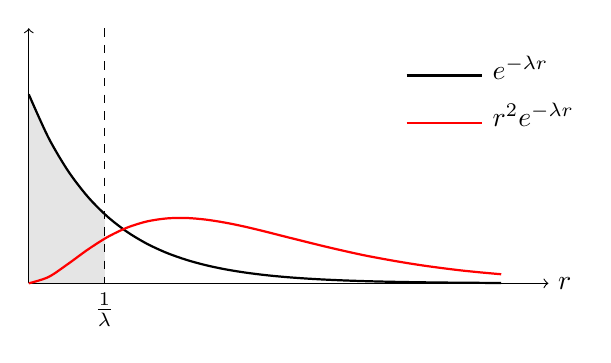
\begin{tikzpicture}[scale=1.2]
        \filldraw[gray!20!] (0,0) -- (0,2) -- plot[smooth, domain=0:0.8] (\x,{2 * exp(-1.25*\x)}) -- (0.8,0) -- cycle;
        \draw[->] (0,0) -- (5.5,0) node[right] {$r$};
        \draw[->] (0,0) -- (0,2.7);
         \draw[thick] plot[smooth, domain=0:5] (\x,{2 * exp(-1.25*\x)});
         \draw[red,thick] plot[smooth, domain=0:5] (\x,{2 * (\x)^2 * exp(-1.25*\x)});
         \draw[dashed] (0.8,2.7) -- (0.8,0) node[below] {$\frac{1}{\lambda}$};
         \draw[thick] (4,2.2) -- (4.8,2.2) node[above=0.1cm, right] {$e^{-\lambda r}$};
         \draw[thick,red] (4,1.7) -- (4.8,1.7) node[black, above=0.1cm,right] {$r^2 e^{-\lambda r}$};
        \end{tikzpicture}
    \end{figure}
\end{soluzione}